
\section{Model Approach }

%%%
%%% SECTION: GOVERNNG EQNS
%%%
\subsection{Governing Equations}

Assume a volume of an incompressible porous medium with porosity, $\phi$, that does not vary in time, containing $N_\mathrm{p}$ immiscible fluid phases.  The volume fraction of each phase is,
\begin{equation}
V_\alpha = \phi S_\alpha,
\end{equation}
where the subscript, $\alpha$, denotes the phase, and $S_\alpha$ is the saturation of that phase such that,
\begin{equation}\label{e:total}
\sum_{\alpha=1}^{N_\mathrm{p}} S_\alpha = 1.
\end{equation}

\subsubsection{Darcy's Law}

Darcy's Law states that for a phase $\alpha$ in a porous medium \cite{bear_1972},
\begin{equation}\label{e:darcy}
\mathbf{q}_\alpha = -\frac{k_{\mathrm{r}\alpha}}{\mu_\alpha}\mathbf{K} \left( \nabla P_\alpha - \rho_\alpha \mathbf{g} \right),
\end{equation}
where $\mathbf{q}_\alpha$ is a volumetric flux rate, known as the Darcy velocity; $k_{\mathrm{r}\alpha}$ is the relative permeability of the phase and is a function of $S_\alpha$; $\mu_\alpha$ is the dynamic viscosity of the fluid phase; $\mathbf{K}$ is a 2nd rank tensor describing the permeability of the porous medium; $P_\alpha$ is the fluid pressure of phase $\alpha$; $\rho_\alpha$ is the mass density of phase $\alpha$; and, $\mathbf{g}$ is the gravitational acceleration vector.

The Darcy velocity can be rewritten in terms of the (interstitial or average) velocity of the fluid, $\mathbf{v}_\alpha$, as,
\begin{equation}
\mathbf{q}_\alpha = V_\alpha \mathbf{v}_\alpha = \phi S_\alpha \mathbf{v}_\alpha.
\end{equation}
Then, we can rewrite Eqn. \ref{e:darcy} as,
\begin{equation}\label{e:darcy2}
S_\alpha \mathbf{\Lambda}_\alpha \mathbf{v}_{\phi\alpha} = - \nabla P_\alpha + \rho_\alpha \mathbf{g},
\end{equation}
with,
\begin{eqnarray}
\mathbf{v}_{\phi\alpha} & = & \phi \mathbf{v}_\alpha,\\
\mathrm{and} \quad \mathbf{\Lambda}_\alpha & = & \frac{\mu_\alpha}{k_{\mathrm{r}\alpha}}\mathbf{K}^{-1}.\label{e:absorption}
\end{eqnarray}

\subsubsection{Mass conservation}

Conservation of mass for each fluid phase implies \cite{bear_1972},
\begin{equation}\label{e:mass}
\phi \frac{\partial}{\partial t}(\rho_\alpha S_\alpha) + \nabla\cdot(\rho_\alpha S_\alpha  \mathbf{v}_{\phi \alpha}) - Q_\alpha = 0,
\end{equation}
where $Q_\alpha$ is a mass flux rate describing sources ($Q_\alpha >0$) or sinks ($Q_\alpha <0$) of phase $\alpha$.

\subsubsection{Fick's Law}

The transport of a conservative substance (e.g.\ salt), with constant mass, in a partially saturated flow can be described by Fick's Law \cite{helmig_1997},
\begin{equation}\label{e:transport}
\phi \frac{\partial}{\partial t}(\rho_\alpha S_\alpha X_\alpha^\kappa) + \nabla \cdot \left( \rho_\alpha S_\alpha X_\alpha^\kappa \mathbf{v}_{\phi\alpha} - \rho_\alpha \mathbf{D}_\alpha^\kappa \nabla X_\alpha^\kappa \right) - R_\alpha^\kappa = 0
\end{equation}
where $R_\alpha^\kappa$ is a source rate for component $\kappa$ in phase $\alpha$; $\mathbf{D}_\alpha^\kappa$ is the 2nd rank hydrodynamic dispersion tensor for component $\kappa$ in phase $\alpha$ (see below); and, $X_\alpha^\kappa$ is the mass fraction of component $\kappa$ in phase $\alpha$ such that,
\begin{equation}
\sum_{\kappa = 1}^{N\mathrm{c\alpha}} X_\alpha^\kappa = 1 \quad \forall\, \alpha,
\end{equation}
and $N_\mathrm{c\alpha}$ is the number of components that phase $\alpha$ can partition into.

It is worth noting that the dispersion tensor, $\mathbf{D}_\alpha^{\kappa}$, may be rewritten in terms of an effective diffusive part and a purely dispersive part, e.g.\ \cite{scheidegger_1961},
\begin{equation}
\mathbf{D}_\alpha^\kappa = (\phi S_\alpha D^{\kappa}_{\mathrm{e} \alpha} + \delta^{\kappa}_{\mathrm{T} \alpha} q_\alpha ) \mathbf{I} + (\delta^{\kappa}_{\mathrm{L} \alpha} - \delta^{\kappa}_{\mathrm{T} \alpha}) \frac{\mathbf{q}_\alpha \mathbf{q}_\alpha}{q_\alpha},
\end{equation}
where $D^{\kappa}_{\mathrm{e} \alpha}$ is the effective molecular diffusion of component $\kappa$ in phase $\alpha$ such that $D^{\kappa}_{\mathrm{e} \alpha} = D^{\kappa}_{\mathrm{m} \alpha} / \tau$, where $D^{\kappa}_{\mathrm{m} \alpha}$ denotes the molecular diffusion coefficient of component $\kappa$ in phase $\alpha$, and $\tau$ is the tortuosity of the porous medium.  The parameters $\delta^{\kappa}_{\mathrm{L} \alpha}$ and $\delta^{\kappa}_{\mathrm{T} \alpha}$ represent the longitudinal and transverse dispersivities of component $\kappa$ in phase $\alpha$, respectively; $\mathbf{I}$ is the 2nd rank unit tensor; and, $q_\alpha = | \mathbf{q}_\alpha |$.

\subsubsection{Fourier's Law}

Assuming local thermal equilibrium, or equivalently rapid heat transfer between the phases, the temperature of all the phases, $T_\alpha$, and the temperature of the porous medium, $T_s$, will be the same i.e.\ $T_\alpha = T_{s} = T$ \cite{hassanizadeh_1993}.  Then, considering the thermal energy of all the fluid phases as well as the porous medium, the energy conservation equation of the system can be described by Fourier's Law as \cite{helmig_1997},
\begin{eqnarray}
& {} & N_\mathrm{p} (1-\phi) c_s \rho_s \frac{\partial T}{\partial t} + N_\mathrm{p} \lambda_s \nabla^2 T \nonumber \\
& {} & {} + \sum_{\alpha = 1}^{N_\mathrm{p}} \left\{ \phi c_\alpha \frac{\partial}{\partial t}(\rho_\alpha S_\alpha T) +  \nabla \cdot \left[ S_\alpha \mathbf{v}_{\phi \alpha} \left(c_\alpha \rho_\alpha T + P_\alpha \right) \right] - U_\alpha \right\} = 0.\label{e:energy}
\end{eqnarray}
Here, $\rho_s$, $c_s$ and $\lambda_s$ are the mass density, the average heat capacity and the heat conductivity, respectively, at constant pressure, of the partially saturated porous medium; $c_\alpha$ is the average heat capacity of phase $\alpha$; and, $U_\alpha$ represents heat flux rate sources or sinks of phase $\alpha$.

%%%
%%% SECTION: CONSTITUTIVE EQNS.
%%%
\subsection{Constitutive Equations}

\subsubsection{Equation of State}

We can express the equation of state as a linearized function of the state variables i.e.\ pressure, temperature and mass fraction of component $\kappa$ in phase $\alpha$, and density of phase $\alpha$,
\begin{equation}\label{e:eos}
\rho_\alpha = \tilde{\rho}_\alpha + \gamma_\alpha^P (P_\alpha - \tilde{P}_\alpha) - \gamma_\alpha^T (T-\tilde{T}_\alpha) + \gamma_\alpha^\kappa (X_\alpha^\kappa - \tilde{X}_\alpha^{\kappa}),
\end{equation}
where parameters with a tilde above them ($\tilde{\ \cdot\ }$) represent an approximation of that parameter in the state space; and,
\begin{eqnarray}
\gamma_\alpha^P & =\ \rho_\alpha \beta_\alpha^P\ = & \frac{\partial \rho_\alpha}{\partial P_\alpha}, \label{e:gammaP}\\
\gamma_\alpha^T & =\ \rho_\alpha \beta_\alpha^T\ = & - \frac{\partial \rho_\alpha}{\partial T}, \label{e:gammaT}\\
\mathrm{and} \quad \gamma_\alpha^\kappa & =\ \rho_\alpha \beta_\alpha^\kappa\ = & \frac{\partial \rho_\alpha}{\partial {X_\alpha^\kappa}}\label{e:gammaX},
\end{eqnarray}
with $\beta_\alpha^P$, $\beta_\alpha^T$ and $\beta_\alpha^\kappa$ representing the compressibility coefficient, thermal expansion coefficient and the coefficient of volume expansion due to component $\kappa$ in phase $\alpha$, respectively.

\subsubsection{Capillary Pressure and Relative Permeability}

The capillary pressure, $P_{\mathrm{c} \alpha \gamma}$, relates the interfacial tension between two phases, $\alpha$ and $\gamma$, in the porous material as,
\begin{equation}\label{e:capillary}
P_{\mathrm{c} \alpha \gamma} = P_\alpha - P_\gamma,
\end{equation}
where $P_\alpha$ is the pressure of the non-wetting phase and $P_\gamma$ is the pressure of the wetting phase. The capillary pressure is usually expressed as a monotonic function of the saturation of the wetting phase (i.e.\ $S_\gamma$), and may be obtained from empirical data, or by using an analytical model such as that of Brooks and Corey \cite{brooks_1964} or Van Genuchten \cite{vangenuchten_1980} in the case of two-phase flow.

Likewise, the relative permeability of a phase, $k_{\mathrm{r}\alpha}$, is dependent on the saturation of that phase, and possibly the saturation of other phases if $N_\mathrm{p} > 2$.  $k_{\mathrm{r}\alpha}$ indicates the perturbation of that phase due to the presence of the other phases and may also be obtained from empirical data or by using an analytical model.  In any case, for all $\alpha$,
\begin{equation}
0 \leq k_{\mathrm{r}\alpha} \leq 1.
\end{equation}

%%%
%%% SECTION: NUMERICAL MODEL FOR COMPRESSIBLE 2-PHASE FLOW
%%%
\subsection{Numerical Model for Compressible Two-Phase Flow}

We consider a system of just two compressible, immiscible fluids (i.e.\ $N_\mathrm{p} = 2$), a wetting phase (hereafter subscripted $w$) and a non-wetting phase (hereafter subscripted $n$).  We assume negligible solute concentration changes and neglible temperature changes, thus reducing  Eqn. \ref{e:eos} to,
\begin{equation}\label{e:eos2}
\rho_\alpha = \tilde{\rho}_\alpha + \gamma_\alpha^P (P_\alpha - \tilde{P}_\alpha).
\end{equation}

\subsubsection{Temporal discretization}\label{s:t_discretization}

We use a backward (implicit) Euler method to discretize the time derivatives in Eqn. \ref{e:mass},
\begin{equation}
\frac{\phi}{\Delta t} S^n_\alpha \left( \rho^{n+1}_\alpha-\rho^n_\alpha \right) + \frac{\phi}{\Delta t} \rho^n_\alpha \left( S^{n+1}_\alpha-S^n_\alpha \right) + \nabla \cdot \left( \tilde{\rho}^{n+1}_\alpha \tilde{S}^{n+1}_\alpha \mathbf{v}^{n+1}_{\phi \alpha} \right) - Q^{n+1}_\alpha = 0,
\end{equation}
where $\Delta t$ is a fixed time increment; variables with a tilde above them ($\tilde{\ \cdot\ }$) are calculated explicitly using a Picard (fixed point) iteration method (e.g.\ see Chapter 9 of Press \textit{et al.}, \cite{press_2008}); and, superscripts denote time level.

Dividing this equation by the mass density of the phase at the current time level, $\rho^n_\alpha$, summing over the phases, and making use of Eqn. \ref{e:total} we get,
\begin{equation}\label{e:t_discretization}
\sum_{\alpha = w,n} \frac{1}{\rho^n_\alpha} \left[ \frac{\phi}{\Delta t} \rho^{n+1}_\alpha S^n_\alpha + \nabla \cdot \left( \tilde{\rho}^{n+1}_\alpha \tilde{S}^{n+1}_\alpha \mathbf{v}^{n+1}_{\phi \alpha} \right) - Q^{n+1}_\alpha \right] - \frac{\phi}{\Delta t} = 0.
\end{equation}

Finally, substituting Eqn. \ref{e:eos2} into Eqn. \ref{e:t_discretization} to eliminate $\rho^{n+1}_\alpha$ we get,
\begin{equation}\label{e:cty}
\sum_{\alpha = w,n} \frac{1}{\rho^n_\alpha} \left\{ \frac{\phi}{\Delta t} S^n_\alpha \left[ \tilde{\rho}^{n+1}_\alpha + \gamma_\alpha^P \left( P^{n+1}_\alpha - \tilde{P}^{n+1}_\alpha \right) \right] + \nabla \cdot \left( \tilde{\rho}^{n+1}_\alpha \tilde{S}^{n+1}_\alpha \mathbf{v}^{n+1}_{\phi \alpha} \right) - Q^{n+1}_\alpha \right\} - \frac{\phi}{\Delta t} = 0.
\end{equation}

This equation can be rewritten in terms of the explicit variables, $P^{n+1}_\alpha$ and $\mathbf{v}^{n+1}_{\phi \alpha}$, as,
\begin{eqnarray}
\frac{\phi}{\Delta t} \sum_{\alpha = w,n} \frac{1}{\rho^n_\alpha} \gamma^P_\alpha S^n_\alpha P^{n+1}_\alpha + \sum_{\alpha = w,n} \frac{1}{\rho^n_\alpha} \nabla \cdot \left( \tilde{\rho}^{n+1}_\alpha \tilde{S}^{n+1}_\alpha \mathbf{v}_{\phi \alpha}^{n+1} \right) {} & = & \nonumber \\
\frac{\phi}{\Delta t} - \sum_{\alpha = w,n} \frac{1}{\rho^n_\alpha} \left[ \frac{\phi}{\Delta t} S^n_\alpha \left( \tilde{\rho}^{n+1}_\alpha - \gamma^P_\alpha \tilde{P}^{n+1}_\alpha \right) - Q^{n+1}_\alpha \right] & {} & \label{e:cty_t}
\end{eqnarray}

Likewise, the temporal discretization of Eqn. \ref{e:darcy2} at time level $(n+1)$ may be written as,
\begin{equation}\label{e:darcy_t}
\tilde{S}^{n+1}_\alpha \tilde{\mathbf{\Lambda}}^{n+1}_\alpha \mathbf{v}^{n+1}_{\phi\alpha} +\left( \nabla  - \gamma_\alpha^P \mathbf{g} \right) P^{n+1}_\alpha = (\tilde{\rho}^{n+1}_\alpha - \gamma_\alpha^P \tilde{P}^{n+1}_\alpha) \mathbf{g}.
\end{equation}

\subsubsection{Spatial discretization}\label{s:x_discretization}

To discretize Eqns. \ref{e:cty_t} and \ref{e:darcy_t} we assume a finite-element mesh such that the velocity field is discretized with $\mathcal{N}$ discontinuous piecewise-linear (P1$_\mathrm{DG}$) degrees-of-freedom and the pressure field is discretised with $\mathcal{M}$ continuous quadratic (P2) degrees-of-freedom (see Figure \ref{f:discretization}a) as introduced by Cotter \textit{et al.} \cite{cotter_2007}, i.e.
\begin{equation}
\mathbf{v}^n_{\phi \alpha} = \sum_{j=1}^\mathcal{N} \hat{\mathbf{v}}^n_{\phi \alpha,j} N_j \quad \mathrm{and} \quad P^n_\alpha = \sum_{j=1}^\mathcal{M} \hat{P}^n_{\alpha,j} M_j.
\end{equation}

\begin{figure}[h]
\vbox{
\hbox{\hspace{1cm}
  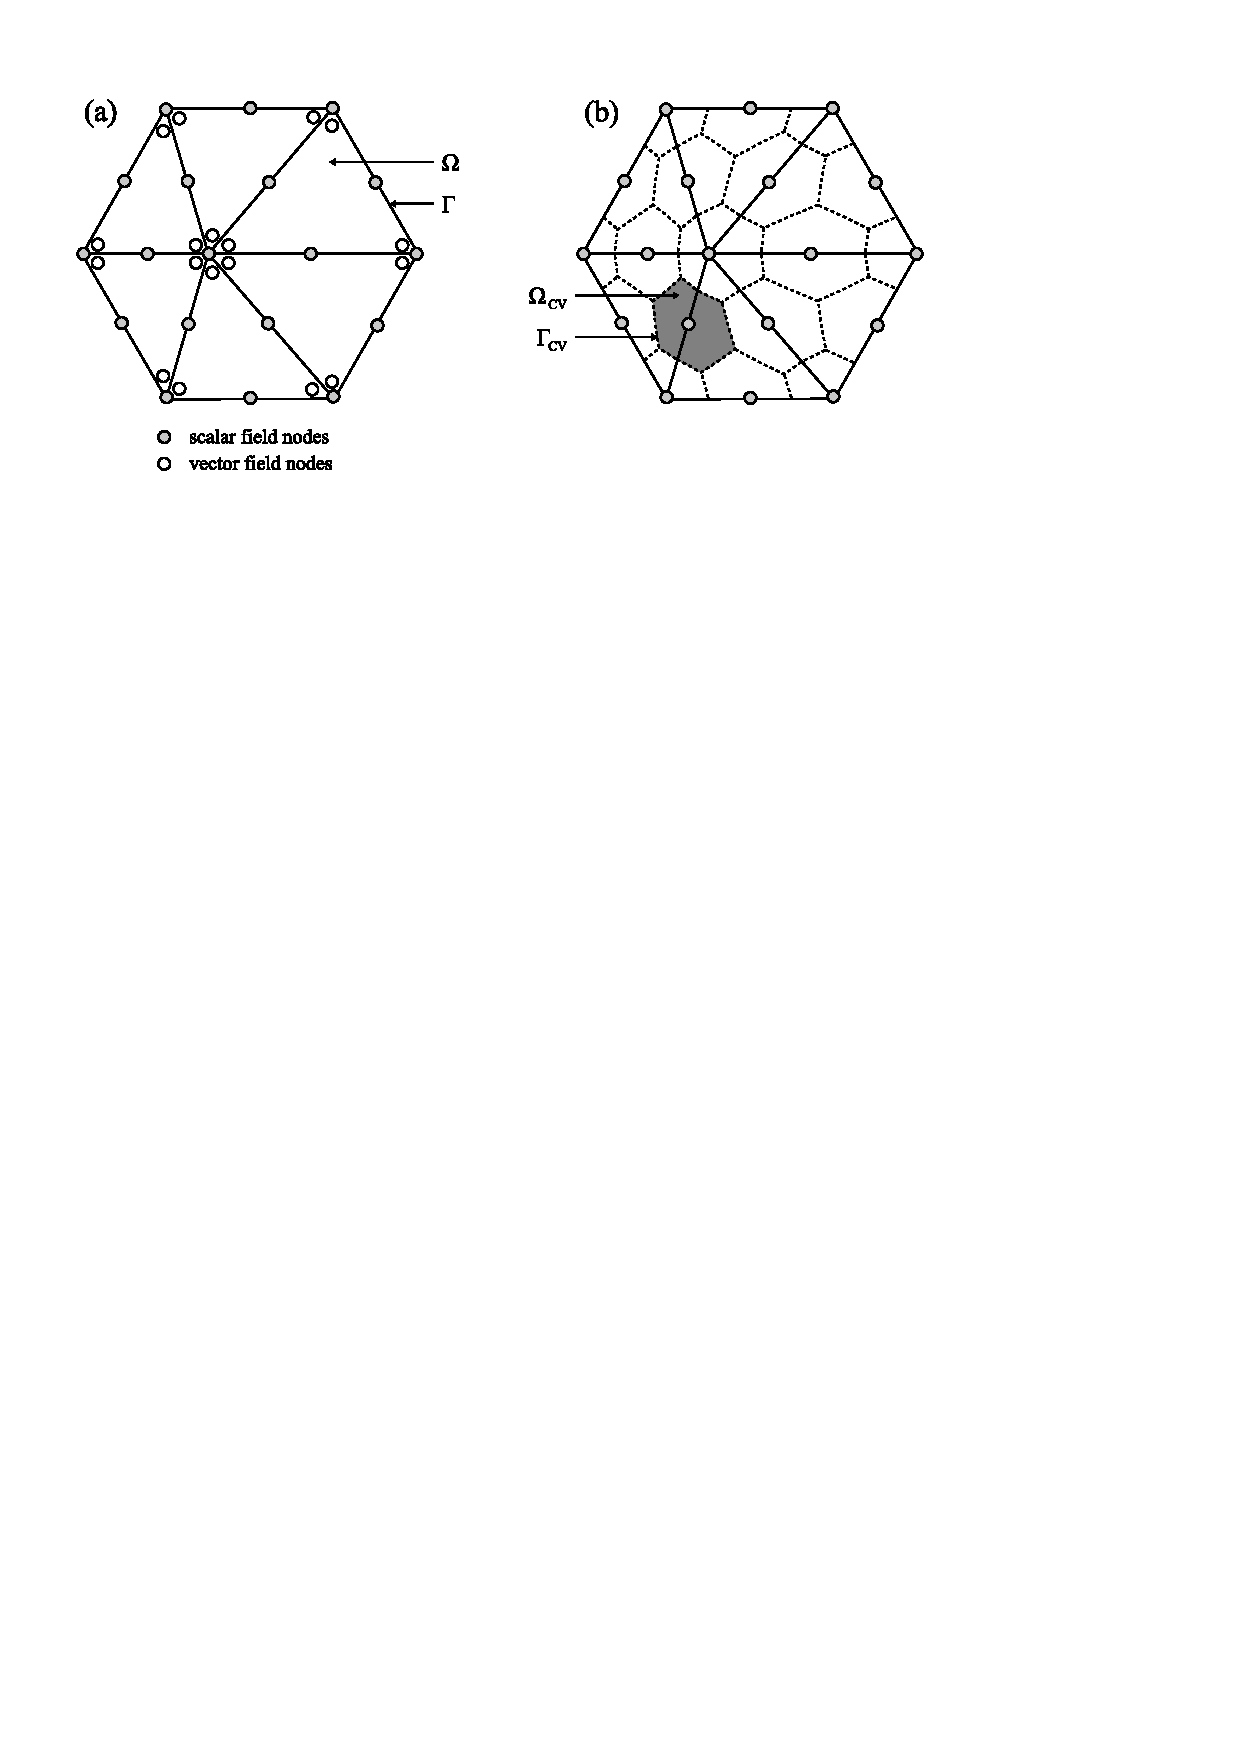
\includegraphics[width=15.0cm,height=19.cm]{./figures/discretization}}
\vspace{-14cm}}
%    \epsfig{file=figures/discretization.eps}
    \caption[]{(a) Example of discretization scheme used in formulation involving P1$_\mathrm{DG}$-P2 elements \cite{cotter_2007}.  Shaded nodes represent degrees-of-freedom for the scalar field (i.e.\ $P_\alpha$) whilst white nodes represent degrees-of-freedom for the vector field (i.e.\ $\mathbf{v}_{\phi \alpha}$).  $\Omega$ is the volume of the domain and $\Gamma$ is its bounding surface.  (b) Control volumes of the same elements, outlined by dashed lines.  $\Omega_\mathrm{CV}$ is the volume of the control volume and $\Gamma_\mathrm{CV}$ is its bounding surface.\label{f:discretization}}
\end{figure}

Then, multiplying Eqn. \ref{e:darcy_t} for each phase by the basis function $N_i$ and integrating over the entire volume of the system, $\Omega$, we get the following matrix equation:
\begin{equation}\label{e:darcy_matrix}
\tilde{\mathbf{A}}^{n+1} \mathbf{v}^{n+1} + \mathbf{B} \mathbf{p}^{n+1} = \tilde{\mathbf{h}}^{n+1},
\end{equation}
where,
\begin{eqnarray}
\mathbf{v}^{n+1} & = & \left[ \hat{\mathbf{v}}^{n+1}_{\phi w} \quad \hat{\mathbf{v}}^{n+1}_{\phi n} \right]^T,\\
\mathbf{p}^{n+1} & = & \left[ \hat{P}^{n+1}_w \quad \hat{P}^{n+1}_n \right]^T,\\
\tilde{\mathrm{A}}^{n+1}_{i,j} & = & \int_\Omega N_i \left[ \begin{array}{c c}
\tilde{S}^{n+1}_w \tilde{\mathbf{\Lambda}}^{n+1}_w & 0 \vspace*{1mm}\\
0 & \tilde{S}^{n+1}_n \tilde{\mathbf{\Lambda}}^{n+1}_n
\end{array} \right] N_j\: d\Omega,\\
\mathrm{B}_{i,j} & = & \int_\Omega N_i \left[ \begin{array}{c c}
\nabla - \gamma^P_w \mathbf{g} & 0 \vspace*{1mm}\\
0 & \nabla - \gamma^P_n \mathbf{g}
\end{array} \right] M_j\: d\Omega,\\
\mathrm{and} \quad \tilde{\mathrm{h}}^{n+1}_{i} & = & \int_\Omega N_i \left[ \begin{array}{c}
(\tilde{\rho}^{n+1}_w - \gamma_w^P \tilde{P}^{n+1}_w) \mathbf{g} \vspace*{2mm}\\
(\tilde{\rho}^{n+1}_n - \gamma_n^P \tilde{P}^{n+1}_n) \mathbf{g}
\end{array} \right] d\Omega.
\end{eqnarray}

Now we consider control volumes, $\Omega_\mathrm{CV}$, with bounding surfaces $\Gamma_\mathrm{CV}$, around each node (see Figure \ref{f:discretization}b), such that,
\begin{equation}
\Omega = \sum_i \Omega_{\mathrm{CV}_i}\quad \mathrm{and} \quad P^n_\alpha = \sum_{j=1}^\mathcal{X} \hat{P}^n_{\alpha,j} \chi_j
\end{equation}
where $\chi_j$ is a basis function that is unity on the control volume and zero elsewhere.  We also enforce $\sum_\alpha S_\alpha = 1$ in each control volume as per Eqn. \ref{e:total}.  Then, multiplying Eqn. \ref{e:cty_t} by the basis function $\chi_i$ and integrating over the control volumes we get the following matrix equation:
\begin{equation}\label{e:cty_matrix}
(\mathbf{M}^n)^T \mathbf{p}^{n+1} + (\tilde{\mathbf{C}}^{n+1})^T \mathbf{v}^{n+1} = \phi - (\tilde{\mathbf{r}}^{n+1})^T \mathbf{1}
\end{equation}
where,
\begin{eqnarray}
\mathrm{M}^n_{i,j} & = & \int_{\Omega_\mathrm{CV}} \chi_i \left[ \begin{array}{c}
\phi \gamma_w^P S^n_w / \rho^n_w \vspace*{2mm}\\
\phi \gamma_n^P S^n_n / \rho^n_n
\end{array} \right] \chi_j\ d\Omega_\mathrm{CV},\\
\tilde{\mathrm{C}}^{n+1}_{i,j} & = & \int_{\Gamma_\mathrm{CV}} \chi_i \left[ \begin{array}{c}
\Delta t\, \tilde{\rho}_w^{n+1} \tilde{S}_w^{n+1} \mathbf{n} / \rho^n_w \vspace*{2mm}\\
\Delta t\, \tilde{\rho}_n^{n+1} \tilde{S}_n^{n+1} \mathbf{n} / \rho^n_n
\end{array} \right] N_j\ d\Gamma_\mathrm{CV},\\
\tilde{\mathrm{r}}^{n+1}_i & = & \int_{\Omega_\mathrm{CV}} \chi_i \left[ \begin{array}{c}
\left\{ \phi S^n_w \left( \tilde{\rho}^{n+1}_w - \gamma^P_w \tilde{P}^{n+1}_w \right) - \Delta t\, Q^{n+1}_w \right\} / \rho^n_w \vspace*{2mm}\\
\left\{ \phi S^n_n \left( \tilde{\rho}^{n+1}_n - \gamma^P_n \tilde{P}^{n+1}_n \right) - \Delta t\, Q^{n+1}_n \right\} / \rho^n_n
\end{array} \right] d\Omega_\mathrm{CV},\\
\mathrm{and} \quad \mathbf{1} & = & \left[ 1\quad 1 \right]^T.
\end{eqnarray}

\subsubsection{Numerical model}

Combining Eqns. \ref{e:darcy_matrix} and \ref{e:cty_matrix} we get,
\begin{equation}
\left[ \begin{array}{c c}
\tilde{\mathbf{A}}^{n+1} & \mathbf{B}\\
(\tilde{\mathbf{C}}^{n+1})^T & (\mathbf{M}^n)^T
\end{array} \right]
\left[ \begin{array}{c}
\mathbf{v}^{n+1}\\
\mathbf{p}^{n+1}
\end{array} \right] =
\left[ \begin{array}{c}
\tilde{\mathbf{h}}\\
\phi - (\tilde{\mathbf{r}}^{n+1})^T \mathbf{1}
\end{array} \right].
\end{equation}
This equation together with Eqns. \ref{e:total} and \ref{e:eos2} (for each of the phases), and appropriate means of calculating $k_{\mathrm{r}w}(S^n_w)$ and $k_{\mathrm{r}n}(S^n_n)$ in Eqn. \ref{e:absorption}, constitutes our numerical model for compressible two-phase fluid flow in a porous medium.

%%%
%%% SECTI0ON: TEST CASES
\subsection{Test cases}

\subsubsection{Buckley-Leverett problem}

\begin{itemize}
\item Example of isothermal multiphase flow.
\item Displacement of oil by water in 1D / 2D.
\item No gravity.
\item No capillary pressure.
\item No dispersion.
\item Comparison with analytical solution.
\end{itemize}

\subsubsection{McWhorter problem}

\begin{itemize}
\item Example of isothermal multiphase flow.
\item Displacement of oil by water in 1D / 2D.
\item No gravity.
\item Inclusion of capillary pressure.
\item Comparison with quasi-analytical solution.
\end{itemize}

\subsubsection{Five-spot waterflood problem}

\begin{itemize}
\item Example of isothermal multiphase flow.
\item Displacement of oil by water in 2D.
\item One injector, one producer; or, Two injectors, two producers.
\item No gravity.
\item Water front shape and diffusivity allows comparison of different numerical techniques.
\end{itemize}

\subsubsection{Heat pipe simulation}

\begin{itemize}
\item Example of non-isothermal multiphase/multicomponent flow.
\item Influence of heat flux on water-steam system.
\item Inclusion of advection, conduction diffusion and capillary effects.
\item Comparison with semi-analytical solution.
\end{itemize}
